\documentclass[12pt]{article}
\usepackage{algos-tasks}

\begin{document}
\task[regular]{Trapezoidal Tiling}

\begin{question}
Let $n$ be a power of two. An equilateral triangle is partitioned into smaller equilateral triangles by parallel lines dividing each of its sides into $n > 1$ equal segments. The topmost equilateral triangle is chopped off (indicated in solid black in the diagram below). We want to tile the remaining equilateral triangles with trapezoids, each of which is composed of three equilateral triangles.

\begin{figure}[H]
\centering
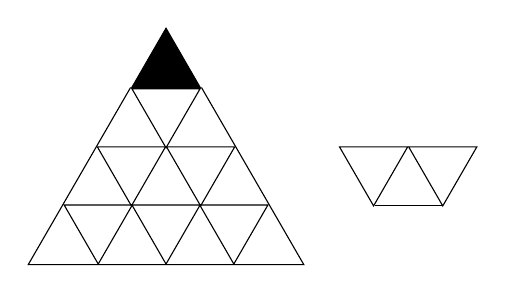
\begin{tikzpicture}[scale = 2]
\def\mytriangle{(90:1)--(210:1)--(-30:1)--cycle}
\coordinate (A) at (-0.875, -0.5);
\coordinate (B) at (-0.225, 0.625);
\coordinate (C) at (0.875, -0.5);
\coordinate (D) at (0.225, 0.625);
\draw (D) -- (C) -- (A) -- (B);
\draw[yshift=14,yscale = -1, scale=0.25] \mytriangle;
\draw[yshift = 3.5, xshift = -6.25,yscale = -1, scale=0.25] \mytriangle;
\draw[yshift = 3.5, xshift = 6.25,yscale = -1, scale=0.25] \mytriangle;
\draw[yshift = -7, xshift = -12.25,yscale = -1, scale=0.25] \mytriangle;
\draw[yshift = -7, xshift = 12.25,yscale = -1, scale=0.25] \mytriangle;
\draw[yshift = -7, xshift = 0,yscale = -1, scale=0.25] \mytriangle;
\draw[yshift = 21.375, xshift = 0, scale=0.25, fill=black] \mytriangle;

\draw[yshift = 3.5, xshift = 50,yscale = -1, scale=0.25] \mytriangle;
\draw[yshift = 3.5, xshift = 37.5,yscale = -1, scale=0.25] \mytriangle;

\coordinate (E) at (1.325,-0.125);
\coordinate (F) at (1.75,-0.125);

\draw (E) -- (F);
\end{tikzpicture}
\label{fig:enter-label}
\end{figure}

Design a divide and conquer algorithm to tile the equilateral triangles with trapzedoids. Justify the correctness of the algorithm and analyse its time complexity.
\begin{itemize}
\item Every equilateral triangle must be covered by at least one trapezoid.
\item No equilateral triangle may be tiled by more than one trapezoid.
\end{itemize}

{\bfseries Note.} {\em A tiling always exists.}
\end{question}
\begin{rubric}
\begin{itemize}
    \item Your response should describe the steps followed to execute the algorithm in simple English. Do not write a program, and do not transcribe a program back to written English.
    
    You \textbf{must} prove the correctness of your algorithm.
    
    You \textbf{must} justify that your algorithm runs in time complexity that you claim.

    \item Course materials such as lectures and tutorials don't require attribution, but making explicit reference to similar ideas is still helpful to show your understanding.
\end{itemize}
Expected response length: around one page.
\end{rubric}

\begin{solution}
\end{solution}

\begin{attribution}
\end{attribution}

\end{document}